\documentclass{standalone}
\usepackage{circuitikz,siunitx}
\usetikzlibrary{shadings,decorations.pathmorphing,arrows.meta,patterns}

\begin{document}
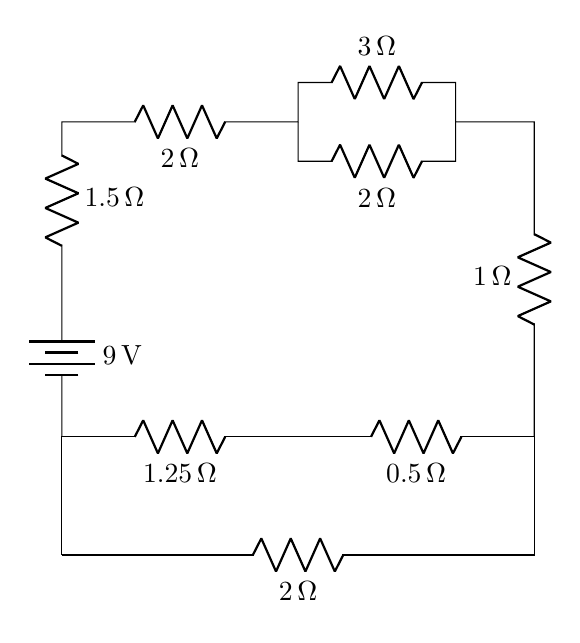
\begin{tikzpicture}
    \draw (0,0) 
      to[R,l_=\SI{2}{\ohm}]      ++( 6, 0)
      to                         ++(0,1.5) coordinate (b)
      to[R,l=\SI{0.5}{\ohm}]     ++(-3, 0)
      to[R,l=\SI{1.25}{\ohm}]    ++(-3, 0) coordinate (a)
      to                         ++( 0,-1.5);
    \draw (b)
      to[R,l=\SI{1}{\ohm}]     ++( 0, 4)
      to                       ++(-1, 0)   coordinate (c)
      to                       ++( 0,0.5)
      to[R,l_=\SI{3}{\ohm}]    ++(-2, 0)
      to                       ++( 0,-0.5) coordinate (d)
      to[R,l=\SI{2}{\ohm}]     ++(-3,0)
      to[R,l=\SI{1.5}{\ohm}]   ++(0,-2)
      to[battery,l=\SI{9}{\volt}] ++(0,-2);
    \draw (c)
      to                       ++(0,-0.5)
      to[R=\SI{2}{\ohm}]       ++(-2,0)
      to (d);
  \end{tikzpicture}
\end{document}